% !TEX TS-program = xelatex
% !TEX encoding = UTF-8 Unicode

\documentclass[pageno]{jpaper}

\newcommand{\IWreport}{2016}


\widowpenalty=9999

\usepackage{caption}
\usepackage{subcaption}
% \usepackage[normalem]{ulem}
% \usepackage[xcdraw]{xcolor}
\usepackage{fontspec}
\usepackage{titlesec}
\defaultfontfeatures{Ligatures=TeX}
\setmainfont{Merriweather}
\setsansfont{Cabin}
\newfontfamily\myfont{Cabin}
% \usepackage[T1]{times}
\usepackage{paralist}
% \usepackage{dingbat}
\usepackage{amssymb}
\usepackage{multicol}
\usepackage{booktabs}
\usepackage{float}




% \titleformat*{\title}{\Large\bfseries\sffamily}
\titleformat*{\section}{\Large\bfseries\sffamily}
\titleformat*{\subsection}{\large\bfseries\sffamily}
\titleformat*{\subsubsection}{\itshape'\/'\subsubsectionfont}



\begin{document}

\title{\myfont{} Exploring Diagnoses of Alzheimer's\\ Using fMRI and Machine Learning}

\author{Allie Burton\\Advisor: Barbara Engelhardt, Ken Norman}

\date{\today}


\maketitle

\thispagestyle{empty}
\doublespacing{}
\begin{abstract}
    Machine learning is rapidly becoming useful in many contexts, particularly
    in the medical field. This paper explores the usage of functional
    magnetic resonance imaging (fMRI) and machine learning in the diagnoses of
    Alzheimer's over the past six years. The most common machine learning methods
    used in the diagnoses of Alzheimer's are feature selection and classification,
    specifically support vector machines. More recent studies have used lesser known
    or more up-and-coming methods such as Gaussian processes and deep learning.
\end{abstract}

\section{Introduction}

Alzheimer's is a devastating disease that affects more than 5 million Americans
that begins as mild memory loss and progresses to inability to have a
conversation and respond to surroundings.
More than five million Americans suffer from this form of dementia, with a new
diagnosis approximately once a minute. There is currently no cure, but research
is ongoing\cite{AlzheimersAssociation2016,AlzheimersAssociation}. Some recent
efforts involve analyzing functional magnetic resonance imaging (fMRI) with
machine learning techniques such as feature selection and classification.

\section{Background}

\subsection{fMRI}

fMRI is a non-invasive neuroimaging technique used to show the behavior of
the brain during various activities. Unlike structural MRI, which only
shows anatomical features, fMRI uses ``imaging of the endogenous
bold-oxygen-level dependent (BOLD) contrast.'' Neuron activation is
accompanied by an increase in blood flow to the respective
area of the brain\cite{Kvisito}.\ fMRIs are usually taken either while the
person is doing a task or while they are resting, creating what is
referred to as a resting-state fMRI, or rs-fMRI.\@ fMRI is also taken over a
period of time, allowing doctors to see the change in activated brain
areas over the course of a task. The resulting data is represented in
\textbf{voxels}, which are the three-dimensional analogs to pixels, each
representing approximately one million brain cells\cite{Yuhas2012}.\ fMRI studies
generate an enormous amount of data despite the small number of participants, thus
making them ideal candidates for computerized processing\cite{Honorio2012}.

\subsection{Using fMRI to Study Alzheimer's}
\label{sub:Using fMRI to Study Alzheimer's}

There are a number of pros and cons to using fMRI to study Alzheimer's.\ fMRI
is ``non-invasive, radiation-free and and offers a combination of good spatial
and reasonable temporal resolution''\cite{Kvisito}. In addition, many fMRIs can
be taken over the course of a longitudinal study, and because studies involving
fMRI are focused on the events taking place while the images are being created,
it's possible to study the ``hemodynamic correlates of specific behavioral events'',
which are critical to understanding Alzheimer's\cite{Dickerson2008}.

Researchers have also proposed that studying the brain as a network could lead
to new insights on Alzheimer's\cite{Khazaee2015,Li2013}. The features of fMRI,
particularly spatial resolution and BOLD contrast, make it well-suited for
testing these hypotheses.

One of the keys to studying any disease is finding \textbf{biomarkers}.
Biomarkers are ``objective, quantifiable characteristics of biological
processes''\cite{Strimbu}. Biomarkers are key to diagnosis. Some have suggested
that fMRI itself could potentially be a biomarker\cite{Sperling2011,Moradi2015}
Recently, researchers have started to use supervised machine learning methods,
specifically feature selection and classification, to find biomarkers for
Alzheimer's\cite{Orru2012,Ye2011}.

Feature selection is invaluable for processing the huge amount of data produced
by fMRI and incredibly useful for identifying biomarkers. It is also essential
to classification by reducing the dimensionality of the data to a manageable amount
for the classifier, thus improving performance\cite{Ye2011}.

In Alzheimer's fMRI studies, classification is commonly used to separate
participants into either the three categories of healthy controls, those with
mild cognitive impairment (an intermediate stage of mental dysfunction that
causes a higher risk of developing Alzheimer's\cite{Khazaee2015}), and those 
with Alzheimer's; or two categories of healthy controls and those with 
Alzheimer's\cite{Morra2010,Khazaee2015,Ye2011}.
Like many other types of data, classifying fMRI data comes with its own set of challenges.
% TODO: Say something about ``curse of dimensionality''
Unlike typical classification problems with many more samples than features, fMRI data has many
more features than samples because of the small number of participants per study.
In addition, due to the thousands of voxels needed to represent a brain, fMRI data
is very high dimensional.\  fMRI data is also known for producing noisy signals.
% FIXME: explain this!!
Finally, fMRI data suffers from high subject variability. In addition to the
standard differences in brain sizes and shapes, Alzheimer's fMRI data has higher
subject variability because of the effects of the disease, which in its later stages
causes those with it to lose motor control. fMRI is extremely 
sensitive to head motion, which can reduce its already relatively low 
spatial resolution. In addition, ``differences in task performance 
between patient and control groups complicate data interpretation, as 
the ability to perform the task may greatly influence the pattern and 
degree of observed fMRI activity.'' Resting state fMRI can counteract
some of these effects and can be used to study those with more 
advanced stages of the disease~\cite{Kvisito}.
% FIXME: find citation!!
% TODO: talk about the dearth of studies

\section{Search Process}
\label{sec:Search Process}

\subsection{Research Questions}
\label{sub:Research Questions}
The questions motivating my analysis were inspired by Wen et.\ al.\ 2012\cite{Wen2012}.
I wanted to summarize the recent research on diagnosing Alzheimer's disease from
fMRI data using machine learning. Thus, my questions were as follows:

\begin{enumerate}
    \item What machine learning techniques have been used for diagnosis of
    Alzheimer's using fMRI data?
    \item In general, how effective/accurate are machine learning models at
    diagnosing Alzheimer's from fMRI data?
    \item Of the machine learning models currently in use, which (if any) perform
    better than others?
    \item Why do some methods perform better than others?
\end{enumerate}

\subsection{Selected Studies}
\label{sub:Selected Studies}
Studies were included in my analysis if they used machine learning methods in
either preprocessing, feature selection, or final classification. They had to
include a clear description of the methods used and why they were chosen and
a thorough analysis of the results. Only studies that restricted their data to
fMRI were chosen, and of the classes to separate data into, Alzheimer's had to
be one of them. The studies chosen were either empirical or proposals for
automated diagnoses of Alzheimer's with fMRI data.

\section{Results and Discussion}
\label{sec:Results and Discussion}

For this literature review, I reviewed seven studies using fMRI and machine learning
to diagnose Alzheimer's ranging from 2009 to 2016. Two of the studies and the
article were overviews or detailed descriptions of suggested methods for studying
and diagnosing Alzheimer's using machine learning and fMRI.\@ The other six studies
either implemented these frameworks or an adaptation of them or used their own methods.
I will explore these studies categorically based on my research questions.

\subsection{Question 1: What Machine Learning Techniques are being Used?}
\label{sub:Question 1: What Machine Learning Techniques are being Used?}
% TODO: Make pie chart of different machine learning techniques
The studies chosen display a wide array of machine learning methods from naïve
Bayes to neural networks. All of the machine learning methods fell into one of
two categories: feature selection or classification. I found eighteen different
methods of feature selection, listed below:

    \begin{singlespace}
    \begin{multicols}{2}
            \begin{itemize}
                \item Random selection
                \item ReliefF
                \item Voxel activation sum
                \item Voxel activation per class
                \item Kendall tau correlation
                \item Gaussian process covariance function
                \item Fisher score
                \item Forward sequential feature selection
                \item Convolutional neural networks
                \item Threshold split region
                \item Principal components analysis
                \item Independent components analysis
                \item Most discriminative voxels
                \item Most active voxels
                \item $16\times16\times16 mm^3$ cubes
                \item Searchlight
                \item Recursive elimination
                \item Symmetric uncertainty
            \end{itemize}
        \end{multicols}
    \end{singlespace}
Fourteen different types of classifiers were found, listed below:

\begin{table}[!ht]
    \centering
    \caption{Frequencies of Classifiers}
\label{Classifier_frequency}
    \begin{tabular}{@{}|l|l|@{}}
        \toprule
        Classifier           & Frequency \\ \midrule
        \rowcolor[HTML]{C0C0C0}
        SVM                  & 6         \\ \midrule
        Naive Bayes          & 3         \\ \midrule
        \rowcolor[HTML]{C0C0C0}
        Random Forests       & 2         \\ \midrule
        Random Subspace      & 1         \\ \midrule
        \rowcolor[HTML]{C0C0C0}
        Random Linear Oracle & 1         \\ \midrule
        Logistic Regression  & 2         \\ \midrule
        \rowcolor[HTML]{C0C0C0}
        KNN                  & 2         \\ \midrule
        Linear Discriminant  & 3         \\ \midrule
        \rowcolor[HTML]{C0C0C0}
        Quadratic Classifier & 1         \\ \midrule
        Decision Tree        & 1         \\ \midrule
        \rowcolor[HTML]{C0C0C0}
        LeNet-5              & 1         \\ \midrule
        Decision Stump       & 2         \\ \bottomrule
    \end{tabular}
\end{table}

There was no overlap between studies for feature selection methods; however,
there was much more overlap for classifiers. Six different forms of support
vector machines appeared in these studies. The second most popular classifier
were forms of linear discriminants, naïve Bayes, and random forests each 
appearing 3 times. Figure~\ref{fig:figure1} shows this graphically.

\begin{figure}[H]
    \centering
    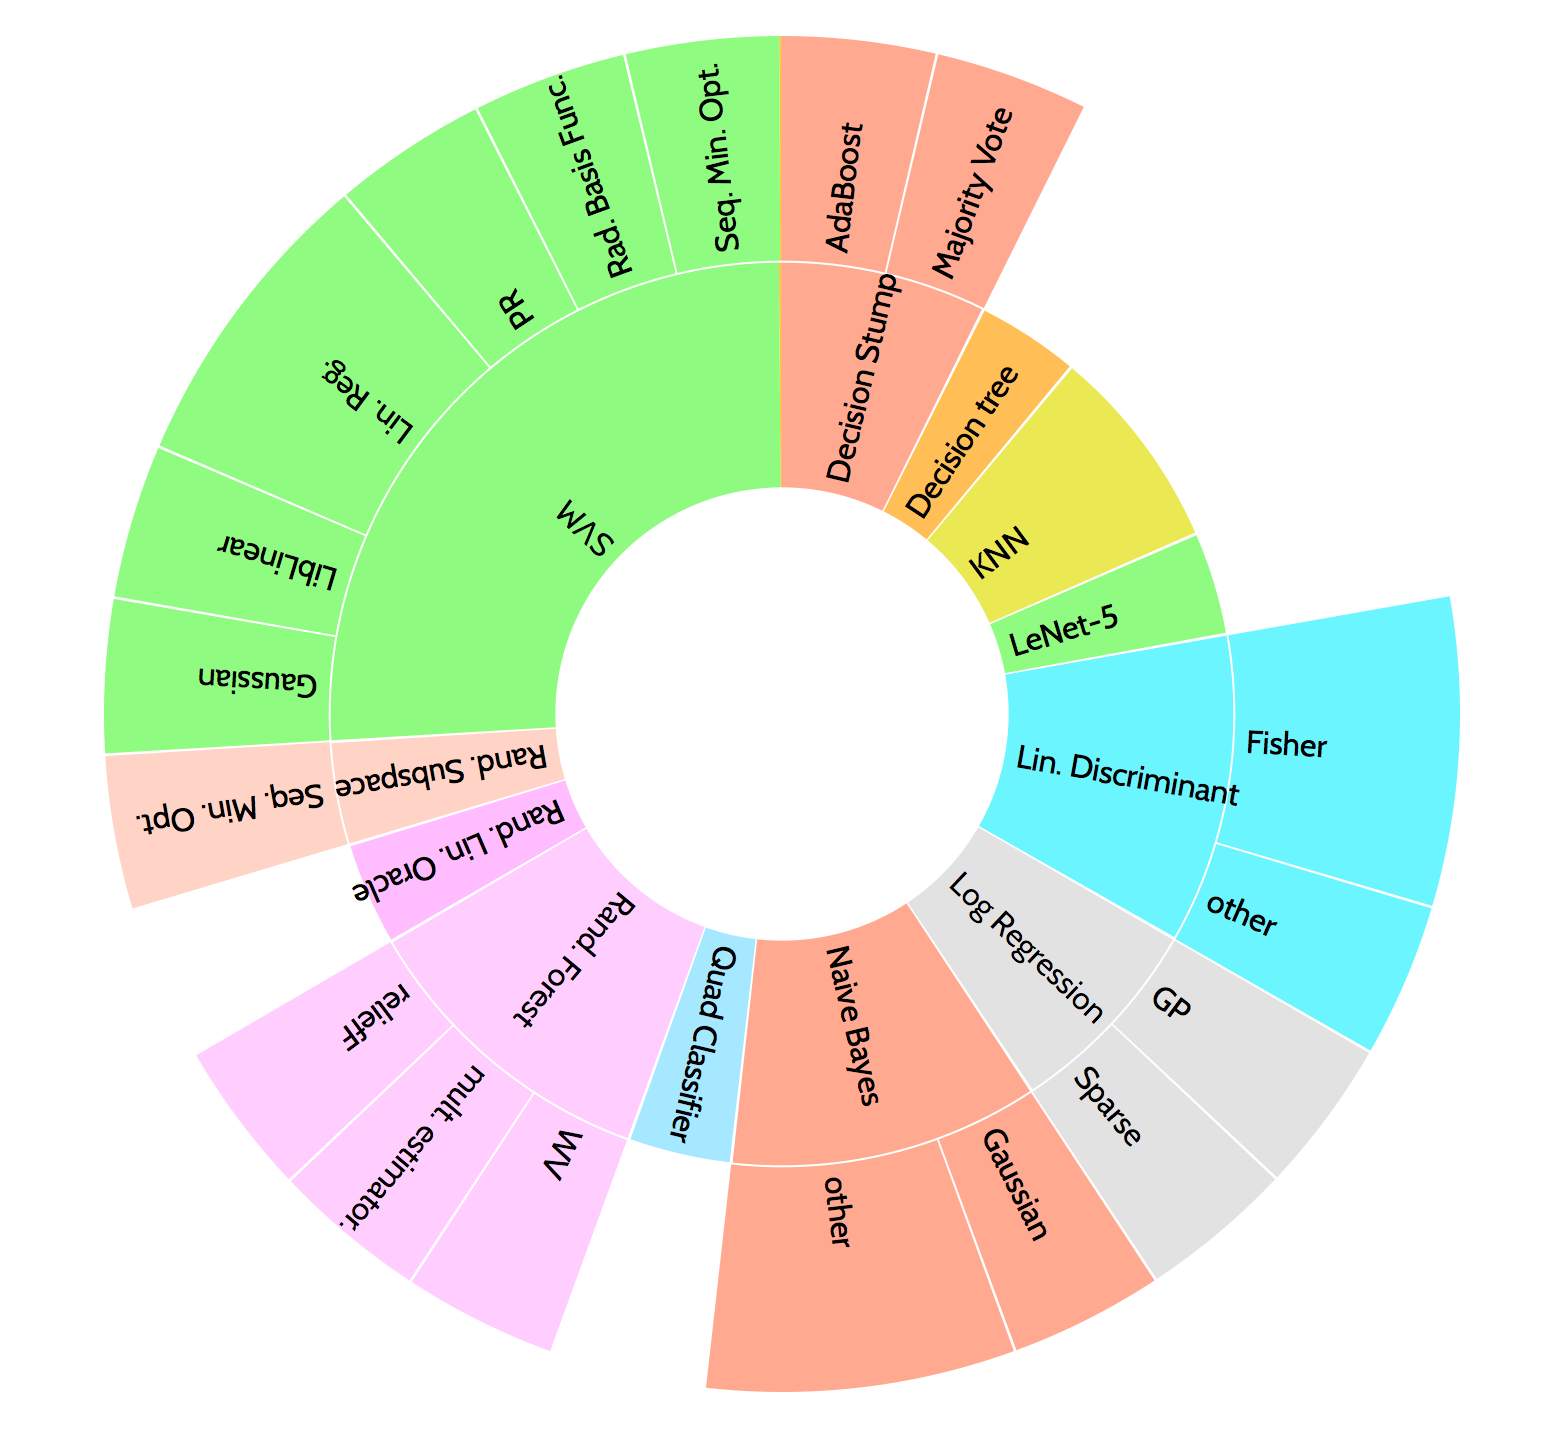
\includegraphics[scale=0.25]{data_visualization/bilevel_partition2.png}
    \caption{Distribution of the Classifiers used in the Studies}
\label{fig:figure1}
\end{figure}
 


\subsection{Question 2: How Effective/Accurate are Machine Learning Models at Diagnosing Alzheimer's?}
\label{sub:Question 2: How Effective/Accurate are Machine Learning Models at Diagnosing Alzheimer's?}
While not perfect, machine learning models actually perform remarkably well at 
predicting Alzheimer's diagnoses. Many of the models achieved over 80\% accuracy
across multiple studies. Figure~\ref{fig:figure2} compares the accuracy of the four 
most popular classifiers from their best performances. SVMs, the most common 
classifier, were regularly accurate more than 90\% of the time.

\begin{figure}[!ht]
    \centering
    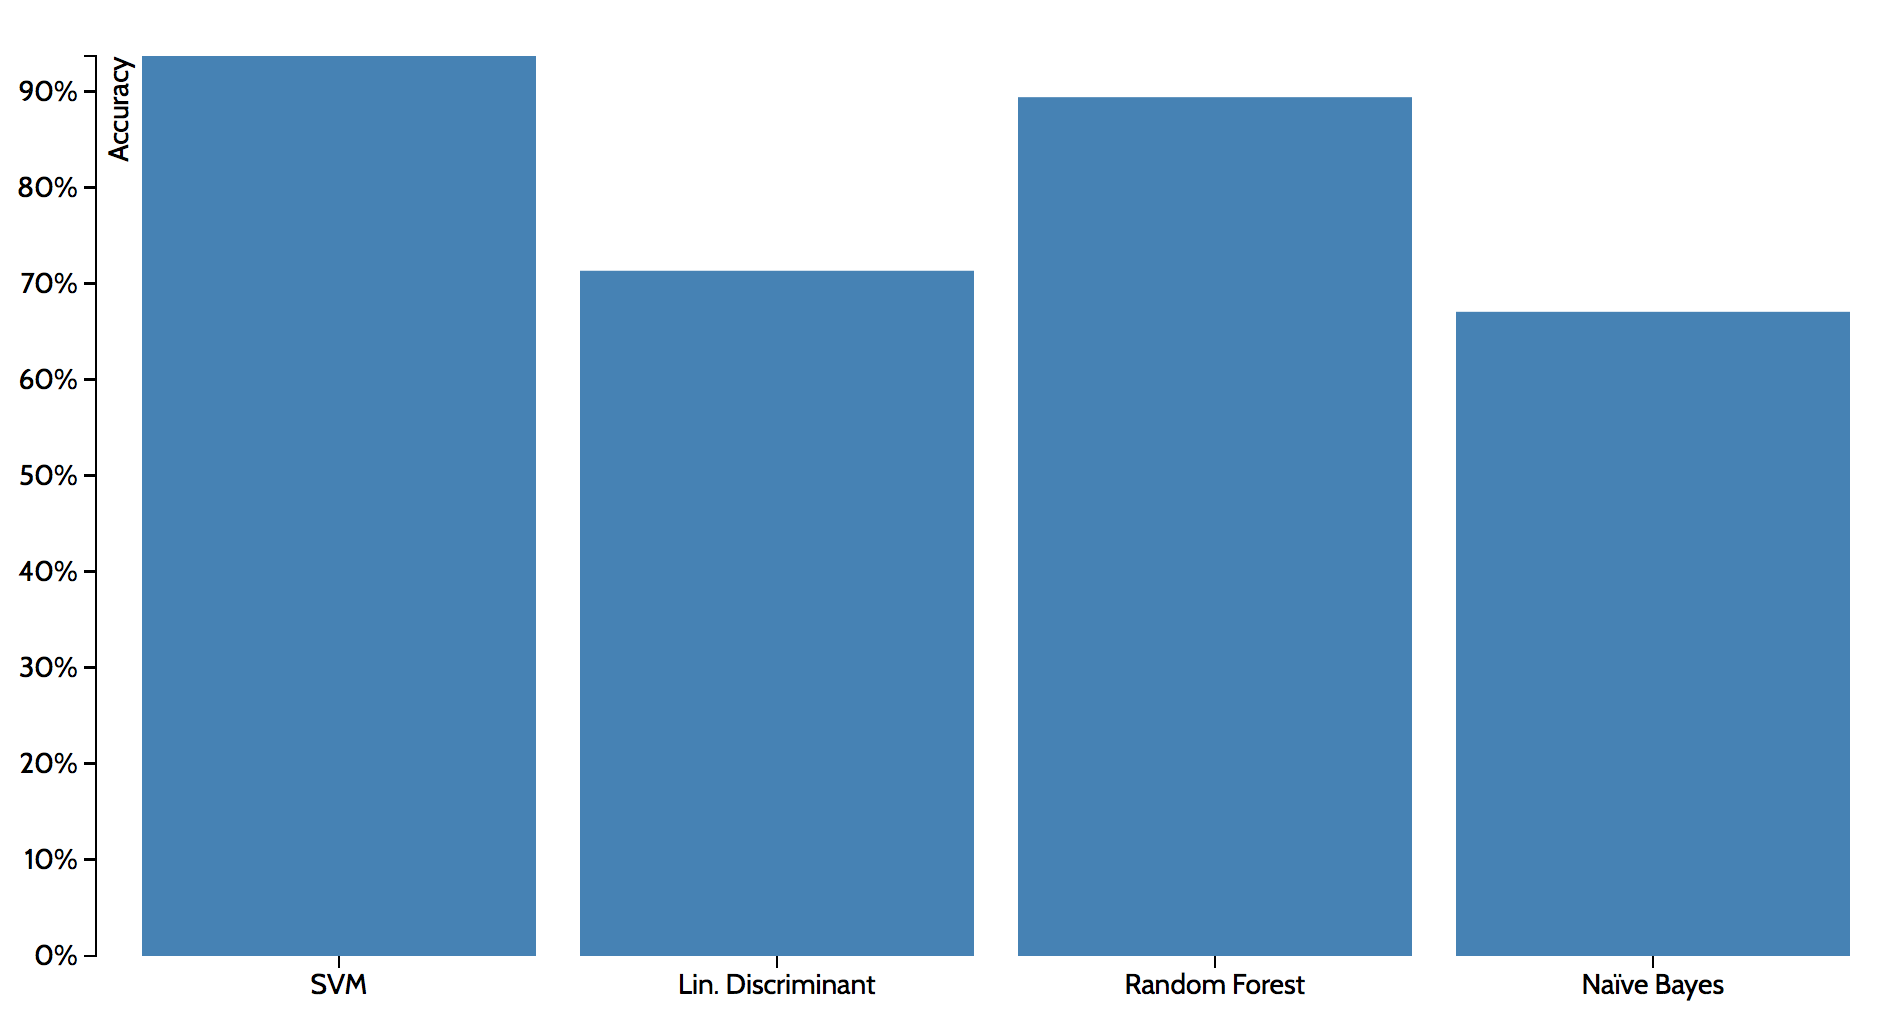
\includegraphics[width=0.5\textwidth]{data_visualization/bar_chart.png}
    \caption{Mean Accuracy of the four most popular classifiers}
\label{fig:figure2}
\end{figure}

\subsection{Question 3: Of currently used models, which ones perform the best?}
\label{sub:Question 3: Of currently used models, which ones perform the best?}
Of the studies reviewed, the most accurate ones for distinguishing Alzheimer's
patients from healthy patients were random forests with improvements from~\cite{Tripoliti2010}, 
the support vector machine with sequential minimal optimization using 25 features 
from~\cite{Armananzas2016} and convolutional neural networks from~\cite{Sarraf2016}, 
which achieved 98\%, 97.14 $\pm$ 2.33\%, and 96.85\% accuracy respectively. 

\subsection{Question 4: Why do some methods perform better than others?}
\label{sub:Question 4: Why do some methods perform better than others?}
Out of the four most common classifiers, naïve Bayes had the worst performance 
consistently. The highest accuracy was in Khazaee et.\ al.~\cite{Khazaee2015}
using all features with feature selection at 80\%. However, the other two studies 
using naïve Bayes had accuracies much closer to Khazaee et.\ al.'s results without 
feature selection: the mean across studies was 54\%, not much better than random 
selection. As explained in Armañanzas, ``This is numerical proof of a biologically
expected phenomenon: the dependence between neighboring voxel signals. Spatially
close voxels will behave in accordance with fashions as large neuronal circuits
activate the whole region.'' Since the efficacy of naïve Bayes is directly 
dependent on the conditional independence of the predictive variables, it makes 
sense that naïve Bayes performs poorly in this case\cite{Armananzas2016}.

Linear discriminant analysis (LDA) performed similarly poorly to naïve Bayes. Like 
naïve Bayes, LDA assumes that the predictive variables are independent and 
additionally assumes that they are normally distributed. The most predictive voxels
for Alzheimer's are neither independent nor normally distributed, so LDA's poor 
performance is understandable. Liong and Foo~\cite{Liong2013} suggest that logistic
regression may have better performance when these assumptions are not met 
``because the results of [logistic regression] are not affected by the degree of 
normality of the independent variables.'' Although this was not supported in the 
data from~\cite{Honorio2012}, Challis et.\ al.'s Gaussian process logistic 
regression performed much more favorably, accurately separating 75\% of healthy 
controls from amnesic-MCI patients and 90\% of amnesic-MCI patients from 
Alzheimer's patients. Furthermore, according to Pereira et.\ al., ``LDA needs to be 
used either in conjunction with extreme feature selection or with dimensionality 
reduction, as otherwise there are typically not enough examples to estimate its 
covariance matrix reliably''\cite{Pereira2009}, so it is possible that LDA could 
have performed better if better features were chosen or if used in conjunction 
a support vector machine for dimensionality reduction.

Random forests performed second best, despite having the highest individual 
performance in Tripoliti et.\ al.'s study~\cite{Tripoliti2010} because of 
improvements such as weighted voting and multiple estimators. The strength of 
random forests is in its ensemble based nature. ``[S]ubstantially different trees
can be constructed from identical training data''~\cite{Armananzas2016}. This 
leads to many different perspectives on the most important features, limited only 
by the number of trees determined to be in the forest.

Support vector machines consistently performed well across all the studies that 
used them. According to~\cite{Armananzas2016}, support vector machines have been 
very popular in fMRI data analysis previously, so it is unsurprising that it was 
also very popular in this subset. ``The ability of SVM to project data to higher 
dimensions in the search of linear separability makes them especially suitable 
for large sized feature spaces'', like voxels from fMRI data. Support vector 
machines do not depend on the assumptions that linear discriminant analysis and 
naïve Bayes depend on, so they are much more flexible and applicable to many 
more classification problems.


\section{Conclusion}


\section{Honor Code}

This represents my own work in accordance with university policies.



\bstctlcite{bstctl:etal, bstctl:nodash, bstctl:simpurl}
\bibliographystyle{IEEEtranS}
\bibliography{references}

\end{document}
